\documentclass{article}

\usepackage[margin=1in]{geometry}
\usepackage{amsmath,amsthm,amssymb}
\usepackage{bbm,enumerate,mathtools}
\usepackage[hidelinks]{hyperref}
\usepackage{tikz}
\usetikzlibrary{matrix, arrows}

\newenvironment{problem}[2][Problem]{\begin{trivlist}
\item[\hskip \labelsep {\bfseries #1}\hskip \labelsep {\bfseries #2.}]}{\end{trivlist}}
\newenvironment{solution}[1][Solution.]{\begin{trivlist}
\item[\hskip \labelsep {\bfseries #1}]}{\end{trivlist}}
\newenvironment{problempart}[1]{\begin{trivlist}\item[\textbf{Part #1.}]}{\end{trivlist}}

\begin{document}

\title{Combinatorics: Homework 4}
\author{Peter Kagey}

\maketitle

% -----------------------------------------------------
% First problem
% -----------------------------------------------------
\begin{problem}{68} $[2]$ \\
  Let $n \geq 1$, and let $f(n)$ be the number of partitions of $n$ such that
  for all $k$, the part $k$ occurs at most $k$ times. Let $g(n)$ be the number
  of partitions of $n$ such that no part has the form $i(i+1)$, i.e., no parts
  equal to $2, 6, 12, 20, \hdots$. Show that $f(n) = g(n)$.
\end{problem}

\begin{solution} \text{} \\
  We can write a generating function for $f$, by \[
    \sum_{n = 1}^\infty f(n)x^n
      = (1 + x)(1 + x^2 + x^4)(1 + x^3 + x^6 + x^9)\hdots
      = \prod_{i=1}^\infty\sum_{j=0}^i x^{ij},
  \] where we choose at most one $1$ in the partition, at most two $2$s in the
  partition, etc.
  Also, the generating function for $g$ is \[
    \sum_{n = 1}^\infty g(n)x^n
    = \frac{1}{{(1 - x)(1-x^2)\hdots}}\prod_{i \geq 1}1 - x^{i(i+1)}
    = \prod_{i \geq 1}\frac{1 - x^{i(i+1)}}{1 - x^i}.
  \]
  \\~\\
  It is enough to show that these two generating functions are equal.
  \\
  In the generating function for $f$, we can write \begin{align*}
    \sum_{j=0}^i x^{ij}
    &= \sum_{j=0}^\infty x^{ij} - \sum_{j=(i+1)}^\infty x^{ij} \\
    &= \frac{1}{1 - x^i} - \frac{x^{i(i + 1)}}{1 - x^i} \\
    &= \frac{1 - x^{i(i+1)}}{1 - x^i}.
  \end{align*}
  Thus the generating function for $f$ can be rewritten as \[
    \sum_{n = 1}^\infty f(n)x^n
    = \prod_{i = 1}^\infty \frac{1 - x^{i(i+1)}}{1 - x^i}
    = \sum_{n = 1}^\infty g(n)x^n,
  \] so $f$ and $g$ are equal.
\end{solution}
\pagebreak
% -----------------------------------------------------
% Second problem
% -----------------------------------------------------
\begin{problem}{69} $[2]$ \\
  Let $f(n)$ denote the number of self-conjugate partitions of $n$ all of whose
  parts are even. Express the generating function $\sum_{n \geq 0}f(n)x^n$ as a
  simple product.
\end{problem}

\begin{solution} \text{} \\
  There exists an ``obvious'' bijection between self-conjugate partitions of $n$
  and self-conjugate partitions of $n$ into even parts. Namely by looking at
  the Ferrer's diagram of a self-conjugate partition, then the bijection $\phi$
  just ``scales up'' the diagram by a factor of two.
  In terms of the partition, each term is doubled and duplicated.
  (This is clearly injective; it is surjective because all self-conjugate
  partitions into even parts must have the parts come in ``pairs'', otherwise
  the conjugate would not have event parts.)
  \\~\\
  For example, \[
    f((4, 2, 1, 1)) = (8, 8, 4, 4, 2, 2, 2, 2)
  \] with the following diagram.
  \[
    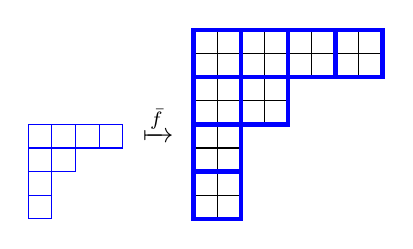
\begin{tikzpicture}[scale=0.3]
      \foreach \x/\y in {
        0/3, 1/3, 2/3, 3/3,
        0/2, 1/2,
        0/1,
        0/0
        } {
        \draw[blue] (\x,\y) rectangle (\x + 1, \y + 1);
        \draw (2*\x + 7, 2*\y) grid (2*\x + 9, 2*\y + 2);
        \draw[ultra thick, blue] (2*\x + 7, 2*\y) rectangle (2*\x + 9, 2*\y + 2);
      }
      \node at (5.5, 4) {$\xmapsto{\bar f}$};
    \end{tikzpicture}
  \]
  Therefore we can reuse the generating function (1.80) that Stanley gives for the
  number of self conguate partitions---only it must be scaled by a factor of
  four: \[
    \sum_{n \geq 0} f(n) x^n
    = (1 + x^4)(1 + x^{12})(1 + x^{20})\hdots
    = \prod_{n \geq 0} 1 + x^{4(2n + 1)}.
  \]
\end{solution}
\pagebreak
% -----------------------------------------------------
% Third problem
% -----------------------------------------------------
\begin{problem}{84} $[2]$ \\
  Show that the number of partitions of $n$ in which each part appears exactly
  $2, 3$, or $5$ times is equal to the number of partitions of $n$ into parts
  congruent to $\pm2$, $\pm3$, $6 \pmod{12}$.
\end{problem}

\begin{solution} \text{} \\
  Let $f(n)$ denote that number of partitions of $n$ in which each part appears
  exactly $2, 3$, or $5$ times, and
  let $g(n)$ denote the number of partitions of $n$ into parts congruent to
  $\pm2$, $\pm3$, $6 \pmod{12}$.
  Then, we have that
  \[
    \sum_{n=0}^\infty f(n)x^n = \prod_{n = 1}^\infty 1 + x^{2n} + x^{3n} + x^{5n},
  \]
  and
  \begin{align*}
    \sum_{n=0}^\infty g(n)x^n
    &= \prod_{n = 1}^\infty\left(1 + x^{2n} + x^{3n} + x^{6n} + x^{9n} + x^{10n} + x^{12n} + \hdots\right) \\
    &= \prod_{n = 1}^\infty\left(
      (1 + x^{2n} + x^{3n} + x^{6n} + x^{9n} + x^{10n})(1 + x^{12n} + x^{24n} + \hdots)
    \right) \\
    &= \prod_{n = 1}^\infty\left(
      \frac{1 + x^{2n} + x^{3n} + x^{6n} + x^{9n} + x^{10n}}{1-x^{12n}}
    \right)
  \end{align*}
  \\~\\
  So if we multiply the generating function of $f$ by this denominator, \[
    \sum_{n=0}^\infty f(n)x^n = \prod_{n = 1}^\infty\frac{(1 + x^{2n} + x^{3n} + x^{5n})(1 - x^{12n})}{1 - x^{12n}},
  \] we can see it is enough to show equality of the generating functions \[
    \prod_{n = 1}^\infty(1 + x^{2n} + x^{3n} + x^{5n})(1 - x^{12n})
    = \prod_{n = 1}^\infty 1 + x^{2n} + x^{3n} + x^{5n} - x^{12n} - x^{14n} - x^{15n} - x^{17n}
  \] and \[
    \prod_{n = 1}^\infty 1 + x^{2n} + x^{3n} + x^{6n} + x^{9n} + x^{10n}.
  \]
  (I couldn't get farther than this.)
\end{solution}
\pagebreak
% -----------------------------------------------------
% Fourth problem
% -----------------------------------------------------
\begin{problem}{85} $[2+]$ \\
  Prove that the number of partitions of $n$ in which no part appears exactly
  once equals the number of partitions of $n$ into parts not congruent to
  $\pm 1 \pmod6$.
\end{problem}

\begin{solution} \text{} \\
  Let $f(n)$ be the number of partitions of $n$ in which no part appears exactly
  once, and let $g(n)$ be the number of partitions of $n$ into parts not
  congruent to $\pm 1 \pmod6$.
  Then the generating function for $f$ is
  \begin{align*}
    \sum_{n=0}^\infty f(n) x^n
    &= \prod_{n=1}^\infty (1 + x^{2n} + x^{3n} + \hdots) \\
    &= \prod_{n=1}^\infty \left(\frac{1}{1-x^n} - x^n\right) \\
    &= \prod_{n=1}^\infty \left(\frac{1 - x^n + x^{2n}}{1-x^n}\right) \\
    &= \prod_{n=1}^\infty \frac{
      \displaystyle\left(\frac{1 + x^{3n}}{1 + x^{n}}\right)
    }{1-x^n} \\
    &= \prod_{n=1}^\infty \frac{1 + x^{3n}}{1-x^{2n}} \\
    &= \left(\prod_{n=1}^\infty \frac{1}{1-x^{2n}}\right)
    \left(\prod_{n=1}^\infty 1 + x^{3n} \right) \\
    &= \left(
      \left(\frac{1}{1-x^{2}}\right)
      \left(\frac{1}{1-x^{4}}\right)
      \left(\frac{1}{1-x^{6}}\right)
      \left(\frac{1}{1-x^{8}}\right)
      \hdots
    \right)
    \left(\prod_{n=1}^\infty 1 + x^{3n} \right).
  \end{align*}
    Now we use Grant Bowling's trick, and break this product up based on
    congruence class,
  \begin{align*}
    \sum_{n=0}^\infty f(n) x^n
    &= \left(\prod_{n=1}^\infty\frac{1}{1-x^{6n - 4}}\right)
    \left(\prod_{n=1}^\infty\frac{1}{1-x^{6n - 2}}\right)
    \left(\prod_{n=1}^\infty\frac{1}{1-x^{6n}}\right)
    \left(\prod_{n=1}^\infty 1 + x^{3n} \right) \\
    &= \left(\prod_{n=1}^\infty\frac{1}{1-x^{6n - 4}}\right)
    \left(\prod_{n=1}^\infty\frac{1}{1-x^{6n - 2}}\right)
    \left(\prod_{n=1}^\infty\frac{1 + x^{3n}}{1-x^{6n}}\right)\\
    &= \left(\prod_{n=1}^\infty\frac{1}{1-x^{6n - 4}}\right)
    \left(\prod_{n=1}^\infty\frac{1}{1-x^{6n - 2}}\right)
    \left(\prod_{n=1}^\infty\frac{1}{1-x^{3n}}\right).
  \end{align*}
  This describes the generating function for $g$ on inspection. \begin{align*}
    \sum_{n=0}^\infty g(n) x^n
  %   &= \prod_{n=1}^\infty (1 + x^{2n} + x^{3n} + x^{4n} + x^{6n} + \hdots) \\
  %   &= \prod_{n=1}^\infty \left((1 + x^{2n} + x^{4n} + x^{6n} + \hdots) + (x^{3n} + x^{9n} + x^{15n} + \hdots)\right) \\
  %   &= \prod_{n=1}^\infty \left(\frac{1}{1-x^{2n}} + \frac{x^{3n}}{1 - x^{6n}}\right)\\
  %   &= \prod_{n=1}^\infty \left(\frac{1 + x^{3n} - x^{5n} - x^{6n}}{1 - x^{2n} - x^{6n} + x^{8n}}\right)
    &= \underbrace{\left(\prod_{n=1}^\infty\frac{1}{1-x^{6n - 4}}\right)}_{\lambda_i \equiv 2 \!\!\!\pmod{6}}
    \underbrace{\left(\prod_{n=1}^\infty\frac{1}{1-x^{6n - 2}}\right)}_{\lambda_i \equiv 4 \!\!\!\pmod{6}}
    \underbrace{\left(\prod_{n=1}^\infty\frac{1}{1-x^{3n}}\right)}_{\lambda_i \equiv 3 \!\!\!\pmod{6}}.
  \end{align*}
  (Use the following procedure: independently choose the number of parts equal
  to $2, 8, 14, \hdots$,
  then choose the number of parts equal to $4, 10, 16, \hdots$,
  and lastly, choose the number of parts equal to $3, 6, 9, \hdots$. Once all
  of these choices are made, there is only one way to order the partition.)
\end{solution}
\pagebreak
% -----------------------------------------------------
% Fifth problem
% -----------------------------------------------------
\begin{problem}{102} $ $
  \begin{enumerate}[(a)]
    \item $[2]$ Let $x$ and $y$ be variables satisfying the commutation relation
    $yx = qxy$, where $q$ commutes with $x$ and $y$. Show that \[
      (x + y)^n = \sum_{k=0}^n \binom{n}{k}_{\!\!q}x^ky^{n-k}.
    \]
    \item $[2]$ Generalize to $(x_1 + x_2 + \hdots + x_m)^n$ where
    $x_ix_j = qx_jx_i$ for $i > j$.

    \item $[2+]$ Generalize further to $(x_1 + x_2 + \hdots + x_m)^n$ where
    $x_ix_j = q_jx_jx_i$ for $i > j$, and where the $q_j$s are variables
    commuting with all the $x_i$s and with each other.
  \end{enumerate}
\end{problem}

\begin{solution} \text{} \\
  (I couldn't make progress on this one.)
\end{solution}
\pagebreak
% -----------------------------------------------------
% Sixth problem
% -----------------------------------------------------
\begin{problem}{125} $[2+]$ \\
  Find the number $f(n)$ of binary sequences $w = a_1a_2\hdots a_k$ (where $k$
  is arbitrary) such that $a_1 = 1$, $a_k=0$ and $\operatorname{inv}(w) = n$.
  For instance, $f(4) = 5$, corresponding to the sequences
  $10000, 11110, 10110, 10010, 1100$. How many of these sequences have exactly
  $j$ $1$s?
\end{problem}

\begin{solution} \text{} \\
  The key insight here is that each binary sequence that meets the criteria
  for $f(n)$ uniquely describes a partition of $n$.

  For example, if we look at the sequences in the example, and we mark the
  number of $0$s that come after each $1$, we get \begin{align}
    1\ 0\ 0\ 0\ 0 &\Rightarrow 4 \\
    1\ 1\ 1\ 1\ 0 &\Rightarrow 1 + 1 + 1 + 1 \\
    1\ 0\ 1\ 1\ 0 &\Rightarrow 2 + 1 + 1 \\
    1\ 0\ 0\ 1\ 0 &\Rightarrow 3 + 1 \\
    1\ 1\ 0\ 0    &\Rightarrow 2 + 2.
  \end{align}
  Therefore $f(n)$ is what Stanley calls $p(n)$, the number of partitions of
  $n$, and the number of sequences with exactly $j$ parts is what Stanley calls
  $p_j(n)$, the number of partitions of $n$ with exactly $j$ parts.
\end{solution}

\end{document}
